\chapter{Marco teórico}

\section{Inteligencia artificial, aprendizaje automático y aprendizaje profundo}

Delimitemos en primer lugar el significado de las diferentes disciplinas utilizadas a la hora de estudiar y desarrollar sistemas de inteligencia artificial. Es frecuente encontrar que términos como \textit{inteligencia artificial} (\textit{Artificial Inteligence}), \textit{aprendizaje automático} (\textit{Machine Learning}) y \textit{aprendizaje profundo} (\textit{Deep Learning}) se utilizan de manera indistinta. Sin embargo, cada uno de ellos tiene un significado específico y es importante distinguirlos para comprender el estado actual de la investigación en el área. Sin embargo, estos conceptos se entienden de forma jerárquica \citep{torresivinalsPythonDeepLearning2020}, donde la inteligencia artificial es el concepto más amplio, que incluye al \textit{aprendizaje automático} y este a su vez al \textit{aprendizaje profundo} (ver Figura \ref{fig:ai_ml_dl}).


\begin{figure}[]
    \caption{Relación AI, ML y DL}
    \centering
    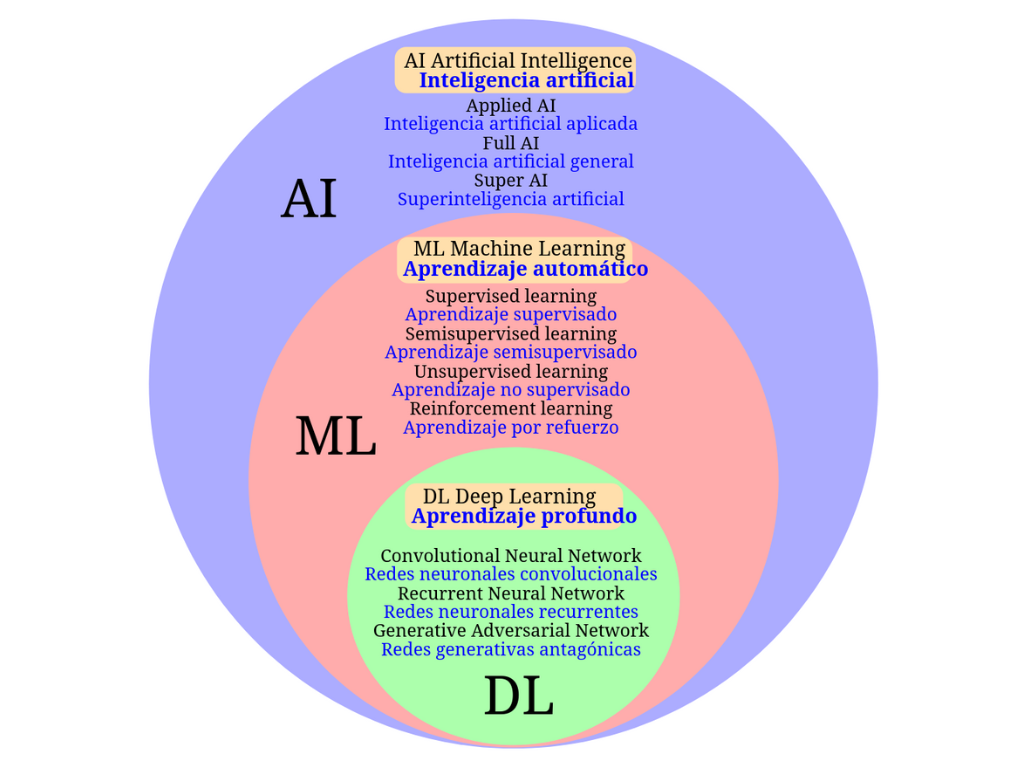
\includegraphics[width=0.8\textwidth]{./figuras/AI_ML_DL.png}
    \source{Jzh2074 \protect\citeyear{jzh2074}, Wikimedia Commons; Wang et al. \protect\citeyear{wang2021promising}.}
    \label{fig:ai_ml_dl}
\end{figure}

% He añadido una imagen de relación AI, ML, DL y AI generativa. Sería interesante modificar lo anterior para hablar también de la IA generativa, que al fin y al cabo es la que nos interesa. La imagen la he sacado de aquí: https://medium.com/@kitkat73275/introduction-to-generative-ai-833c9c467dfa (añadirla a bibliografía y citarla)


Tratemos de delimitar cada uno de estos conceptos.

\subsection{Inteligencia artificial}

La inteligencia artificial es el campo de estudio más antiguo de los tres, y no queda limitado al ámbito computacional. La inteligencia artificial ha sido objeto, en su sentido más amplio, por la filosofía. Los mismos racionalismos y estructuralismos, propios de los sistemas de pensamiento occidentales, están en la base conceptual de la inteligencia artificial. No será, no obstante, hasta el siglo XX donde se comience a plantear de forma explícita la posibilidad matemática de un sistema capaz de generar inteligencia. En 1950, Alan Turing publica su artículo \textit{Computing Machinery and Intelligence} \citep{alan1950a}, donde propone un test para determinar si una máquina es capaz de pensar. Este test, conocido como \textit{Test de Turing}, en la interacción de una entidad humana con una artificial, a través de un terminal de texto como única interfaz. La máquina supera el test si el humano no es capaz de distinguir si la entidad con la que está interactuando es artificial o humana. A este test, a pesar de su escaso rigor y su restricción antropocéntrica del concepto de inteligencia, aún se apela de manera frecuente para valorar la capacidad de sistemas de IA modernos.

Sin embargo, el concepto de inteligencia artificial va más allá de la pura imitación humana, si bien no la excluye. Si tomamos la \emph{racionalidad} como un conjunto de estructuras lógicas, dentro de cuyos sistemas se engloba el pensamiento y racionalidad humanos, no es necesario que la inteligencia artificial se limite en su objetivo a superar el test de Turing. Las diferentes definiciones de inteligencia artificial que se han dado a lo largo de la historia han variado su acento según hayan puesto su mira en la imitación del pensamiento o acción \emph{humanos}, o en el pensamiento y acción \emph{racional} \citep{RussellStuartJ2021AI:A}.

Es a matemáticos como Turing o Curt Gödel a quienes debemos los fundamentos matemáticos de procesos de pensamiento como sistemas computacionales capaces de generar \textit{outputs} racionales a partir de \textit{inputs} arbitrarios. La idea de que el propio cerebro humano es una de las infinitas \emph{máquinas de Turing} posibles \citep{penroseNuevaMenteEmperador2015} ha sido un pensamiento muy atractivo y que ha impulsado la investigación de la IA computacional. Por otra parte, las investigaciones en \textit{procesamiento del lenguaje natural}, entre las que debemos de destacar el concepto de \emph{entropía} de Shannon \citep{shannon1951prediction}, que han ido parejas al desarrollo de los lenguajes de programación de computadoras, están en la base de los modernos sistemas de IA.

\subsection{Machine Learning}

El \textit{Machine Learning}, o \textit{aprendizaje automático}\footnote{En cuanto disciplina de estudio, utilizaremos en lo sucesivo el término \textit{Machine Learning}, en inglés, por ser el más extendido.}, es una rama de la inteligencia artificial que se centra en el estudio de algoritmos y modelos matemáticos que permiten a un sistema computacional aprender de los datos, en lugar de ser explícitamente programado para ello. El \textit{Machine Learning} se basa en la idea de que los sistemas computacionales pueden aprender de los datos, identificar patrones y tomar decisiones con mínima o nula intervención humana. Se podría decir que en el \textit{Machine Learning} el modelo se programa a sí mismo a partir de los datos. Solo el diseño de su arquitectura y la selección de los datos de entrenamiento son tareas humanas ---o ajenas al sistema, ya que esta función podría ser delegada a otro sistema de \textit{Machine Learning} entrenado para ello. El \textit{Machine Learning} ha sido objeto de estudio desde los albores de la computación, pero no hay que olvidar que es un subconjunto de lo que denominamos \textit{inteligencia artificial}, y que no todo sistema inteligente es un sistema de \textit{Machine Learning}.

Como ejemplo de esto último, muchos de los grandes avances en inteligencia artificial vinieron dados por sistemas que no utilizaban \textit{Machine Learning}. El \textit{Deep Blue} de IBM, que en 1997 derrotó al campeón mundial de ajedrez Garry Kasparov, no utilizaba \textit{Machine Learning} \citep{campbellDeepBlue2002}. El \textit{Deep Blue} era un sistema de inteligencia artificial que utilizaba una base de datos de jugadas de ajedrez, y un algoritmo de búsqueda de árbol de juego, para determinar la mejor jugada posible en cada momento. Ejemplos de otros campos que juego son los \emph{sistemas expertos}, que utilizan reglas de inferencia, programadas por humanos conocedores de la materia, para determinar la mejor acción posible en cada momento. Los sistemas expertos son utilizados con éxito en campos como la medicina, la ingeniería o la gestión empresarial.

Pero, ¿en qué consiste el aprendizaje de un sistema de \textit{Machine Learning} y qué se espera de su entrenamiento? El \textit{Machile Learning} intenta buscar una función matemática que pueda explicar un conjunto de datos utilizados para su entreamiento, de modo que después pueda predecir con suficiente fiabilidad y precisión datos no conocidos en la fase de entreamiento. Esta última fase predictiva se denomina fase de \textit{inferencia}. De algún modo, se espera que esa función encontrada en el proceso de entramiento sea una buena aproximación de la función que explica los datos, de modo que el sistema sea capaz de generalizar, análogamente a cómo lo hace el cerebro humano.

Denominamos \textit{modelo} al sistema ya entrenado y con capacidad predictiva. El modelo es el resultado del proceso de entrenamiento, y es el que se utiliza en la fase de inferencia. El modelo puede ser utilizado para predecir datos no conocidos, o para clasificarlos en categorías. En el primer caso, hablamos de \textit{regresión}, y en el segundo de \textit{clasificación}. En el caso de la regresión, el modelo produce un valor numérico, y en el de la clasificación, una categoría. En el caso de la clasificación, el modelo puede ser binario, es decir, que solo puede clasificar en dos categorías, o multiclase, que puede clasificar en más de dos categorías. En el caso de la regresión, el modelo puede ser unidimensional, es decir, que solo produce un valor numérico, o multidimensional, que produce más de un valor numérico.

% Continuar con tipos de Machine Learning, y explicar el aprendizaje supervisado, no supervisado y por refuerzo, citar a torres, y explicar el aprendizaje profundo como un subconjunto del aprendizaje automático.

Los sistemas de \textit{Machine Learning} aprenden de los datos a través de un proceso de \textit{entrenamiento}. En función de la forma en que se le presentan dichos datos y la manera que tiene el sistema de comprobar si su salida es correcta o no, podemos distinguir tres tipos de aprendizaje automático: \textit{aprendizaje supervisado}, \textit{aprendizaje no supervisado} y \textit{aprendizaje por refuerzo} \citep[p. ~38]{torresivinalsPythonDeepLearning2020}. Estamos hablando de \textit{aprendizaje supervisado} cuando los datos que el sistema aprende vienen etiquetados con la respuesta que se espera de él en el momento de la inferencia. A modo de ejemplo, Al sistema se le puede presentar para su entreamiento una colección de imágenes de animales etiquetadas como \textit{gato} y \textit{perro}. Tras el proceso de entreamiento se espera del sistema que en la fase de inferencia, dada una imagen no etiquetada sea capaz de producir una salida que indique si la imagen contiene un gato o un perro. En el \textit{aprendizaje no supervisado} no se etiquetan los datos de entrenamiento, y el sistema debe ser capaz de encontrar patrones en los datos y agruparlos en categorías. En el ejemplo anterior, el sistema no sabría si las imágenes que se le presentan son de gatos o de perros, y debería ser capaz de agruparlas en dos categorías. Por último, en el \textit{aprendizaje por refuerzo} el sistema no recibe datos etiquetados, sino que debe aprender a partir de la interacción con el entorno. Continuando con el mismo ejemplo, el sistema no recibiría imágenes etiquetadas, sino que debería aprender a partir de la interacción con el entorno, y recibiría una recompensa positiva si acierta y una negativa si falla. El sistema debería aprender a partir de estas recompensas a clasificar las imágenes.


\section{Deep Learning}

qué es el Deep Learning, y por qué ha evolucionado tanto en los últimos años, factores: poder computacional, cantidad de datos disponibles, democratización de la computación, mejoras en las arquitecturas y modelos de Deep Learning.

A partir de ahí se explican detalles desde las redes neuronales hasta Transformer, que es el estado del arte actual de deep learning, incluyendo los modelos de lenguaje que nos atañen.


\subsection{Tipos de redes neuronales}
\subsection{Arquitecturas de redes neuronales}
\subsection{Datos y entrenamiento de modelos de \textit{Deep Learning}}

\subsection{La arquitectura Transformer}

En la Figura \ref{fig:transformer_architecture} se puede ver un esquema de la arquitectura \textit{Transformer}.

\begin{figure}[]
    \caption[Aquitectura de Transformer]{Aquitectura de Transformer}
    \centering
    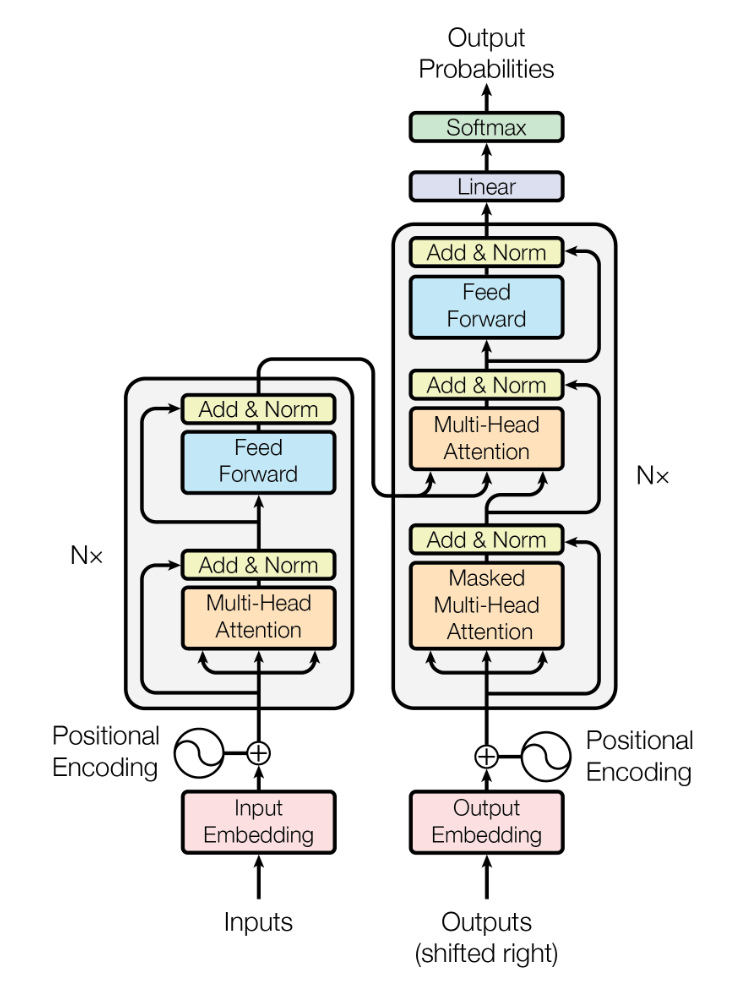
\includegraphics[width=0.4\textwidth]{./figuras/Transformer_architecture.png}
    \source{\cite{vaswaniAttentionAllYou2017}}
    \label{fig:transformer_architecture}
\end{figure}

\section{Modelos de lenguaje}

% Nos centramos en los modelos de lenguaje, para entender su funcionamiento. Importantísimo para comprender el papel de estos en la generación de código.

Un \textit{modelo de lenguaje} no es más que un modelo estadístico que asigna una probabilidad a una secuencia de palabras dada como input. En ese sentido, se reduce a una función matemática \textit{modelada} para imitar la forma en la que se escribe en lenguaje natural. Una forma sencilla de entender qué hace un \textit{modelo de lenguaje} es pensar en un teclado predictivo. Cuando escribimos un mensaje en nuestro teléfono móvil, el teclado predictivo nos sugiere las palabras que más probablemente podrían seguir a las que hemos escrito. Este comportamiento aparentemente inocuo y trivial es el que está detrás de los \textit{modelos de lenguaje}, incluyendo los chatbots más avanzados del momento.

Más técnicamente hablando, un \textit{modelo de lenguaje} devuelve como output la distribución de pobabilidad del siguiente \textit{token}, dada una lista de \textit{tokens} como entrada \citep{GenerationLLMs}. Un \textit{token} es la unidad mínima de información que recibe el \textit{modelo de lenguaje} y equivale, grosso modo, a una palabra\footnote{Un token puede ser una palabra, pero también un signo de puntuación, un número, o cualquier otra unidad mínima de información. En el caso de los modelos de lenguaje, los tokens suelen ser palabras, pero en el caso de los modelos de \textit{Machine Learning} en general, los tokens pueden ser cualquier unidad mínima de información, como por ejemplo los píxeles de una imagen.}. En la Figura \ref{fig:llm_generation} se puede ver un ejemplo de un \textit{modelo de lenguaje} que recibe como input una lista de palabras y devuelve como output la distribución de probabilidad de la siguiente, tras su entreamiento con grandes cantidades de textos en inglés.

\begin{figure}[]
    \caption[Inferencia de \textit{token} de un LLM]{Inferencia de \textit{token} de un LLM}
    \centering
    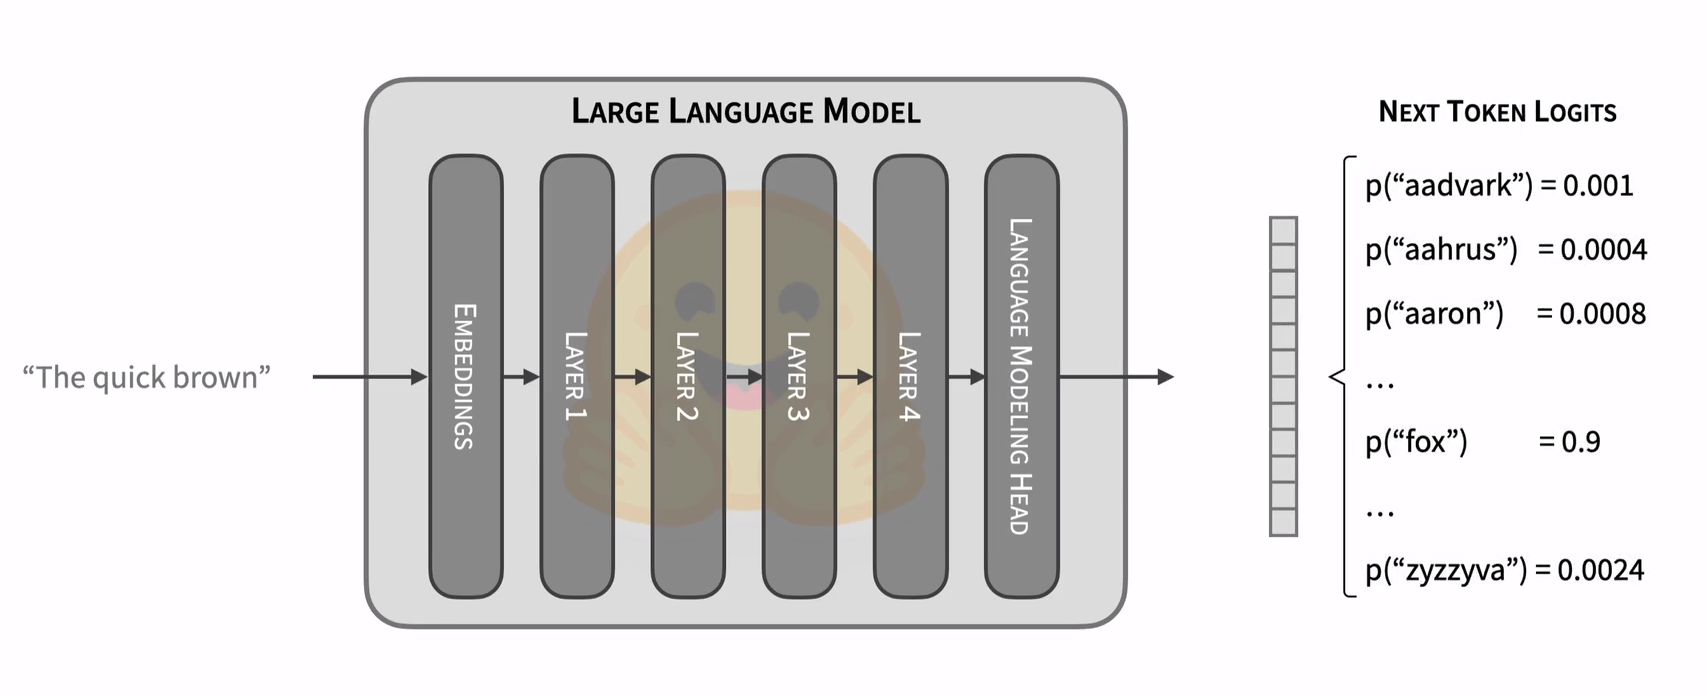
\includegraphics[width=0.9\textwidth]{./figuras/LLM_predice_token.png}
    \source{\cite{GenerationLLMs}}
    \label{fig:llm_generation}
\end{figure}

Los \textit{modelos de lenguaje} no están asociados a una única arquitectura de \textit{Machine Learning}, sino que pueden ser implementados por diversos tipos de redes neuronales, como las redes neuronales recurrentes, las redes neuronales convolucionales, o las redes neuronales Transformer, de las cuales se ha hablado más arriba. En todo caso, el punto de inflexión que ha permitido avances sin precedentes en el mundo del \textit{Machine Learning} ha sido, sin duda alguna, el desarrollo de la arquitectura \textit{Transformer}. 

\subsection{Grandes modelos de lenguaje}

Un \textit{gran modelo de lenguaje} (LLM) es un modelo de lenguaje con un número de parámetros del orden del billón. El primer gran modelo de lenguaje fue \textit{GPT-2}, desarrollado y entrenado por OpenAI en 2019 \citep{radfordLanguageModelsAre2019a}. \textit{GPT-2} fue entrenado con 40 GB de texto de Internet, y alcanzó un tamaño de 1.5 billones de parámetros. \textit{GPT-2} fue entrenado con el objetivo de predecir la siguiente palabra de una secuencia de texto dada, sorprendiendo a la comunidad científica por la calidad de los textos generados, sin precedentes en la historia del \textit{Deep Learning}. A pesar de ello, OpenAI decidió publicar un modelo reducido, por miedo a los posibles usos irresponsables de esta nueva tecnología. El modelo puesto al público constaba de 117 millones de parámetros, el que utilizó para generar los textos de prueba que se pueden ver en la Figura \ref{fig:gpt2_text_generation}. 

\begin{figure}[]
    \caption{Generación de textos por \textit{GPT-2}}
    \centering
    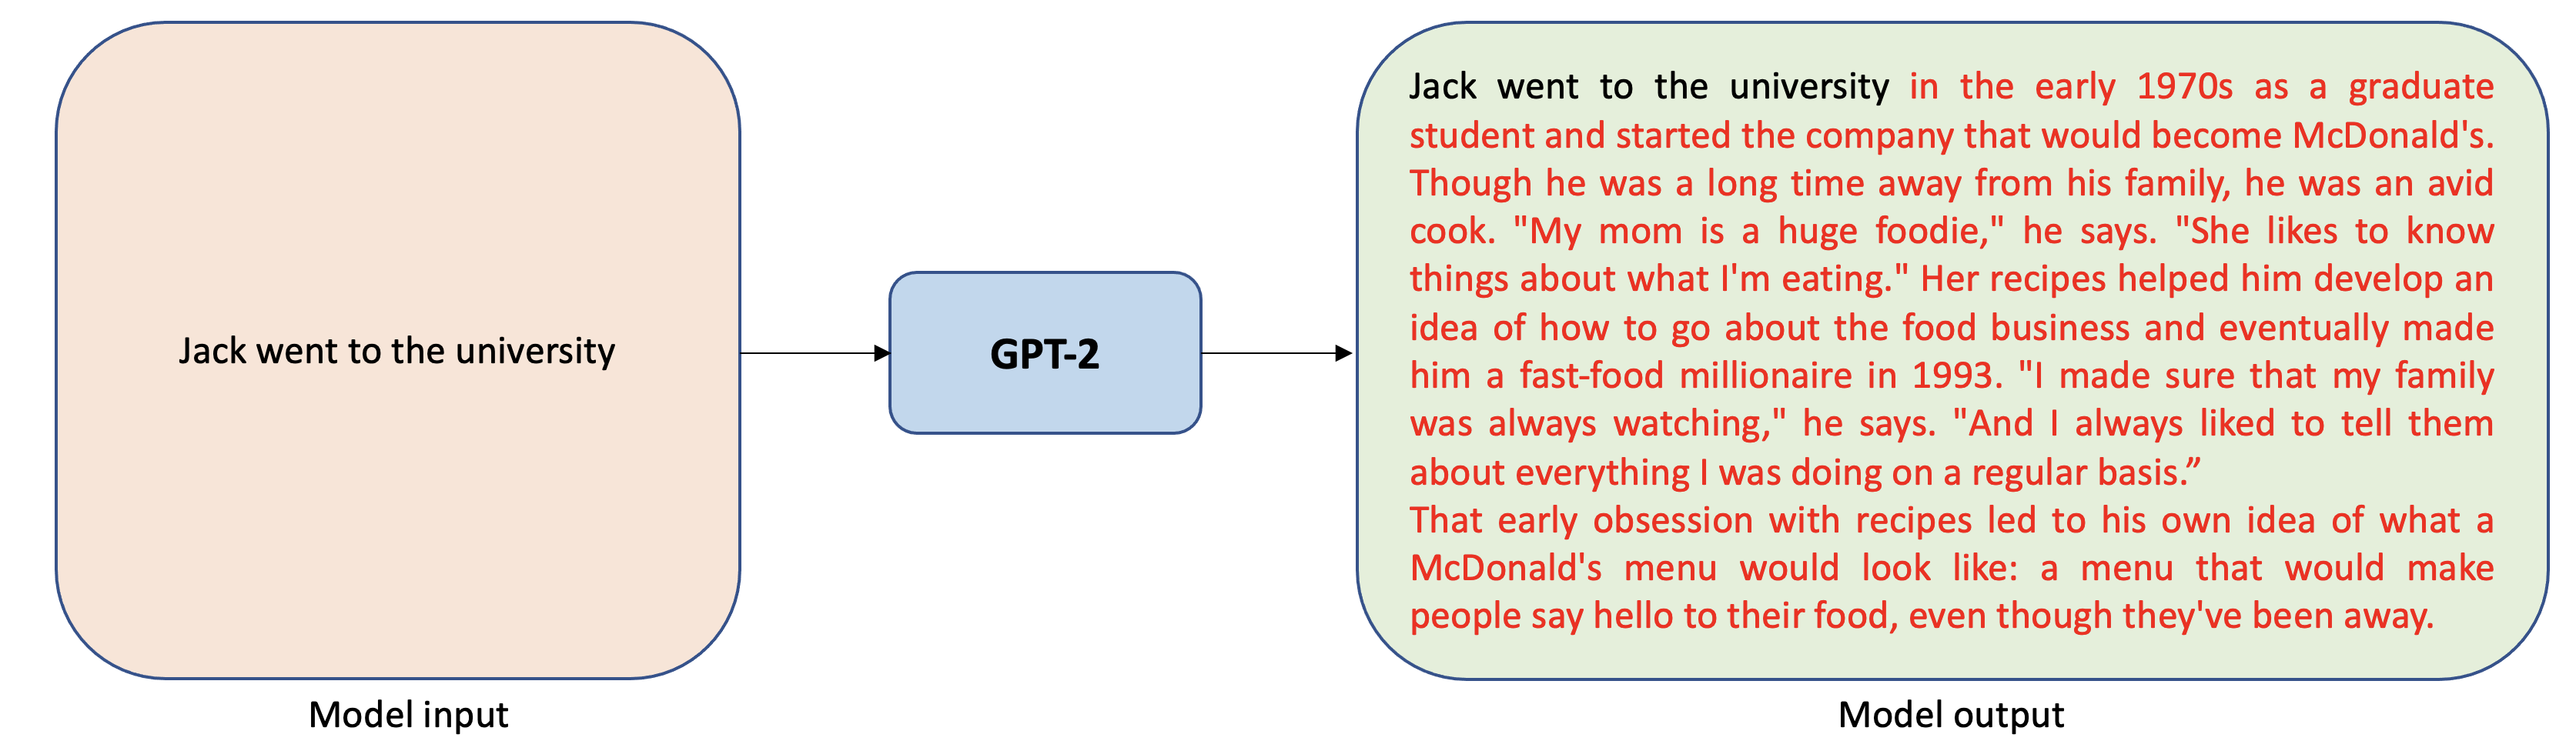
\includegraphics[width=0.9\textwidth]{./figuras/GPT2_text_generation.png}
    \source{\cite{RunTextGeneration2022}}
    \label{fig:gpt2_text_generation}
\end{figure}

Los \textit{grandes modelos de lenguaje} se basan en la arquitectura \textit{Transformer} \citep{vaswaniAttentionAllYou2017}, la cual ha permitido una eficiencia computacional y una escalabilidad de los modelos sin ningún precedente. Desde su aparición en 2017 la escalada por el tamaño de los modelos ha sido exponencial. En la Figura \ref{fig:llm_sizes} se puede comparar el tamaño de diversos LLM a lo largo del tiempo.

\begin{figure}[]
    \caption{Gráfico comparativo de tamaños de LLM}
    \centering
    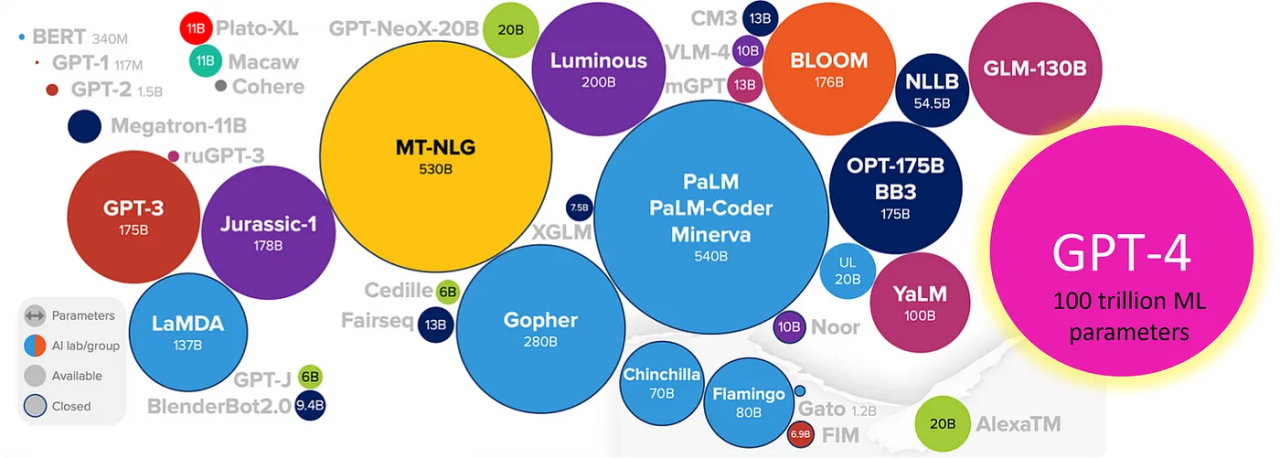
\includegraphics[width=0.9\textwidth]{./figuras/LLMs_sizes.png}
    \source{\cite{ChallengesAssociatedBuilding}}
    \label{fig:llm_sizes}
\end{figure}

\subsection{Modelos prentrenados}
\subsection{Ajuste fino de los modelos}
\subsection{Habilidades emergentes de los modelos de lenguaje}
\subsection{Prompting engineering}
Exponer aquí esta disciplina nueva, y un esquema general de todas las aproximaciones a ello. \citep{LLMPromptingGuide}

